%!TEX root = main.tex
\chapter{Methods and results}
In this section we will outline what methods we have used for conducting the work.
\section{Data preparation}
\subsection{Data import to database}
We imported the many JSON files to a Postgresql database which allowed us to easily manipulate the data using SQL. We created a single table with the schema shown in Table \ref{table:schema_denormalized}. We decided to compute the time and spatial bins on insertion, thus we only had to compute them once. We created indexes on the following features: X.
Initially we created a normalized database with several relations, this we found severely slowed down the performance of our queries. This was due to all our interaction with the data only consisting of READs, after the initial insertion of the data. After removing all relations (denormalizing) our performance significantly improved. {\color{red} evt referer til paper 'Denormalization effects on performance of RDBMS'}.
\begin{table}[htbp]
\centering

\begin{tabular}{|c|c|c|c|c|c|c|c|c|c|c|}
\hline
\textbf{Field name} & \textbf{Field type}    \\
\hline
id                  & SERIAL PRIMARY KEY     \\
\hline
useruuid            & TEXT NOT NULL          \\
\hline
start\_time         & TIMESTAMPTZ NOT NULL   \\
\hline
end\_time           & TIMESTAMPTZ NOT NULL   \\
\hline
location            & GEOGRAPHY(POINT, 4326) \\
\hline
altitude            & INTEGER NOT NULL       \\
\hline
accuracy            & INTEGER NOT NULL       \\
\hline
region              & TEXT                   \\
\hline
country             & TEXT                   \\
\hline
area                & TEXT                   \\
\hline
place               & TEXT                   \\
\hline
time\_bins          & INTEGER{[}{]} NOT NULL \\
\hline
spatial\_bin        & BIGINT NOT NULL        \\
\hline
\end{tabular}
\caption{Denormalized database schema}
\label{table:schema_denormalized}
\end{table}
\subsection{Data export to Numpy arrays}
We created scripts for exportation to numpy arrays for use in the sklearn module. The users were encoded with K values where K = number of users. The countries were encoded with K values where K = number of countries.

\subsubsection{Binning} \label{ssec:binning}
In the following section the term grid cell or spatial bin will be used synonymously and time interval and time bin aswell.
A spatiotemporal co-occurrence between two users is defined as an instance in which they co-occurred in approximately the same time and approximately the same place.
We have partitioned or binned the globe into a discrete grid where the cells span .001\degree of latitude and longitude on each side, and in a discrete time interval of 1-hour.
Thus we say a co-occurrence happens between users A and B if they share the same .001\degree spatial cell C within the same discrete time interval.
 Each grid cell has a unique ID, this is obtained by considering the grid as a matrix and flattening it to a list by traversing from left to right and top to bottom (row-first ordering) and using the list index as an ID. This makes a total possible spatial bin indexes of: $(190\times dec)\times(360\times dec)=68.400.000.000$ with $dec=3$ We calculated the time bins by counting every hour from the start of the day of the earliest date appearing in the dataset, which has the ISO 8601 timestring: "2015-08-09 22:25:33.766+02". The latest day has the ISO 8601 timestring: "2015-12-01 00:59:15.738+01". This leaves us with $2738$ possible time bin IDs. For generating our dataset we count co-occurrences between pairs only once per spatial and time bin.


\subsection{Visualization}
We used Basemap\cite{basemap}, for plotting all the locations at once and and Leaflet\cite{leaflet} for producing interactive maps to visualize the data, we created a map for visualizing the users location traces over time and we created one that allowed us to see all the co-occurrences that happened between a pair of users. We found both location updates and co-occurrences happened very often near Sony properties in Lund\cite{sony_headquarters_sweden_lund}, Kista\cite{sony_headquarters_sweden_kista}, and an Ericsson building in Göteborg\cite{ericsson}, Sweden, and in Tokyo\cite{sony_headquarters_japan}, Japan. Figure \ref{fig:sweden_locations_hexbin} and \ref{fig:japan_locations_hexbin} shows location updates from Sweden and Japan respectively plotted on a map. Figure X shows an example of the co-occurrences visualized for a pair of users ('8d325d9f-9341-4d00-a890-2adaf412e5ca', 'a21d8502-c5cb-4eb5-8b19-b38ea74e9294'). This enabled us to exclude co-occurrences from these locations for the test dataset {\color{red} WHY?}.
\begin{figure}[H]
    \hspace*{-1.0cm}
    \centering
    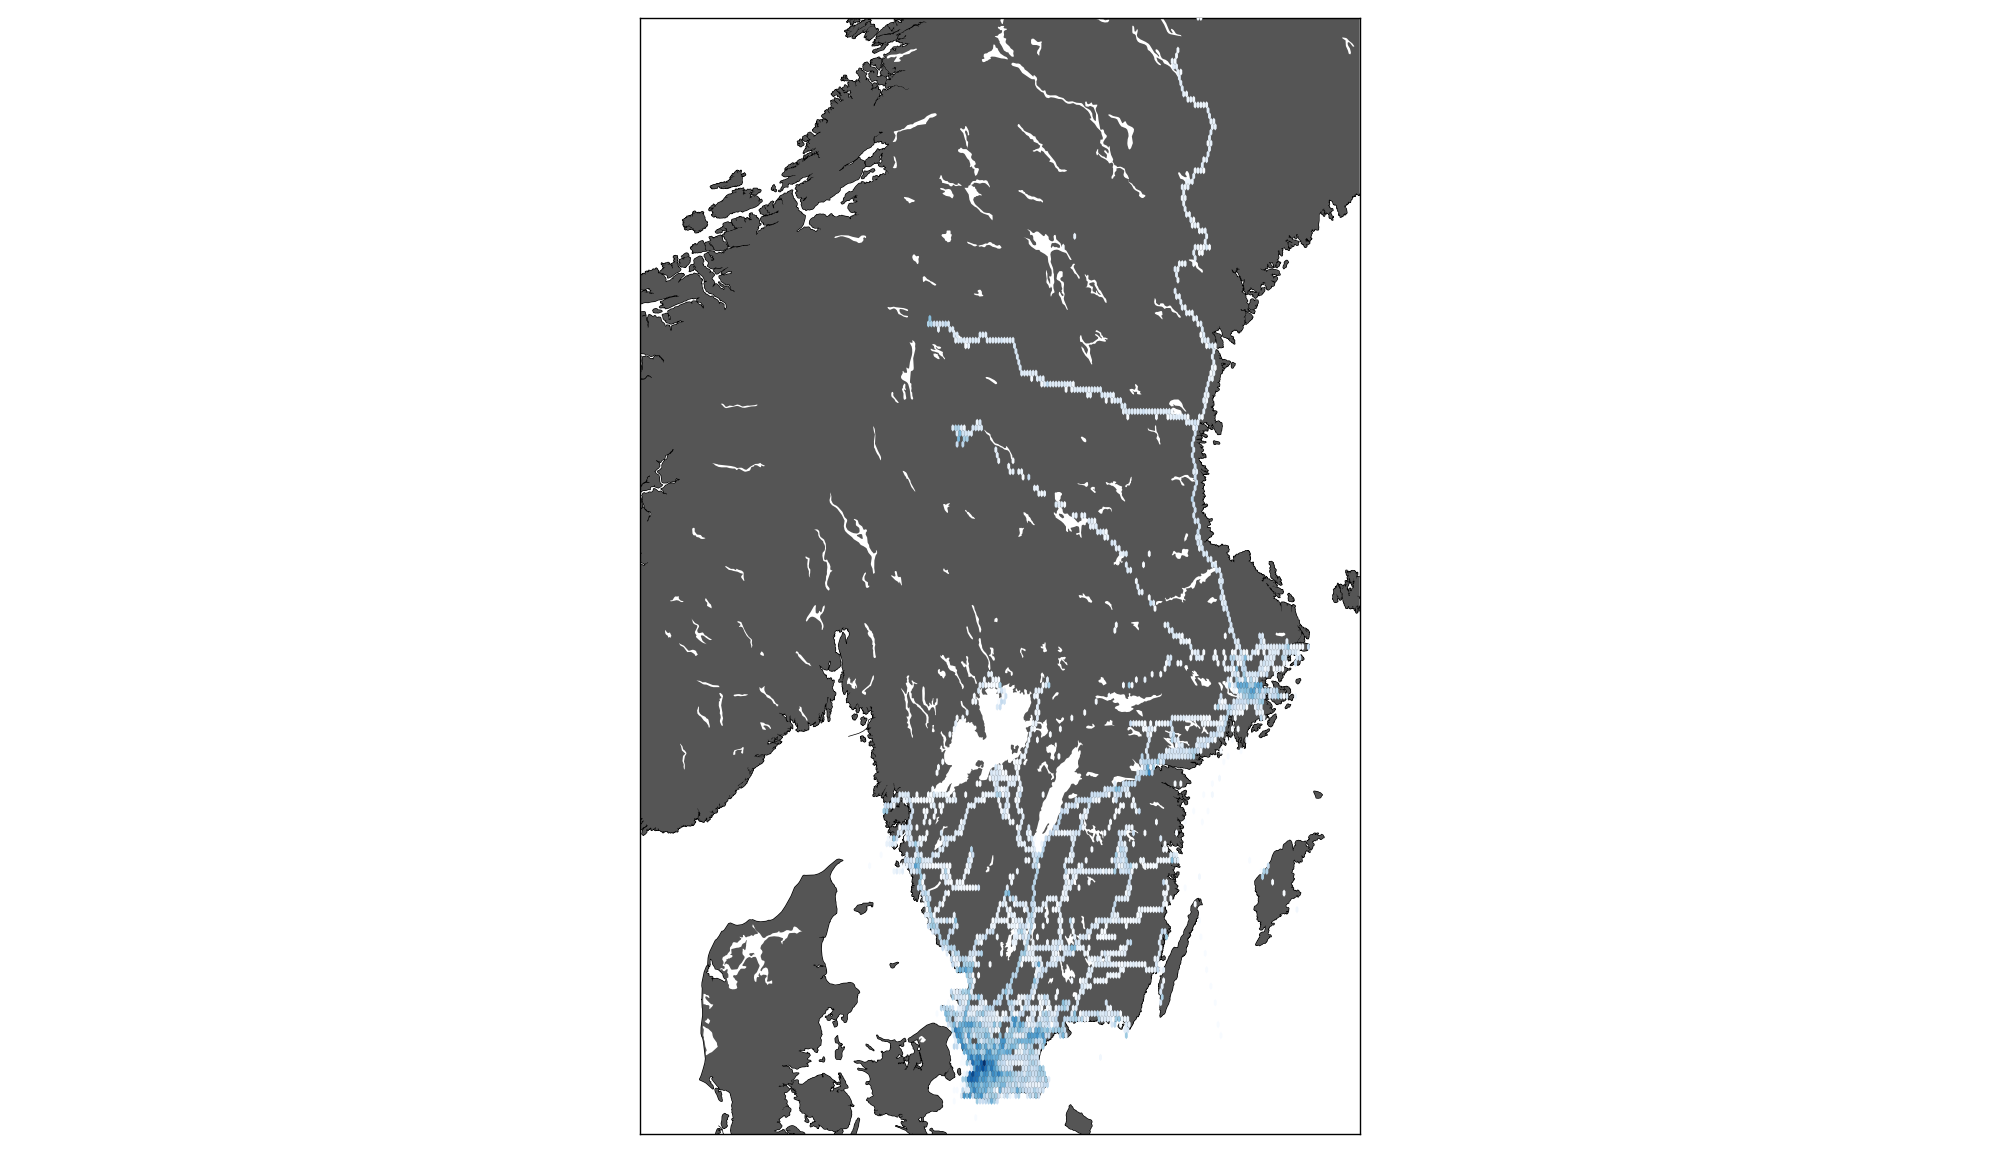
\includegraphics[scale=0.30]{all_locations_sweden}
    \caption{Location updates in Sweden, hexbinned}
    \label{fig:sweden_locations_hexbin}
\end{figure}
\begin{figure}[H]
    \hspace*{-1.0cm}
    \centering
    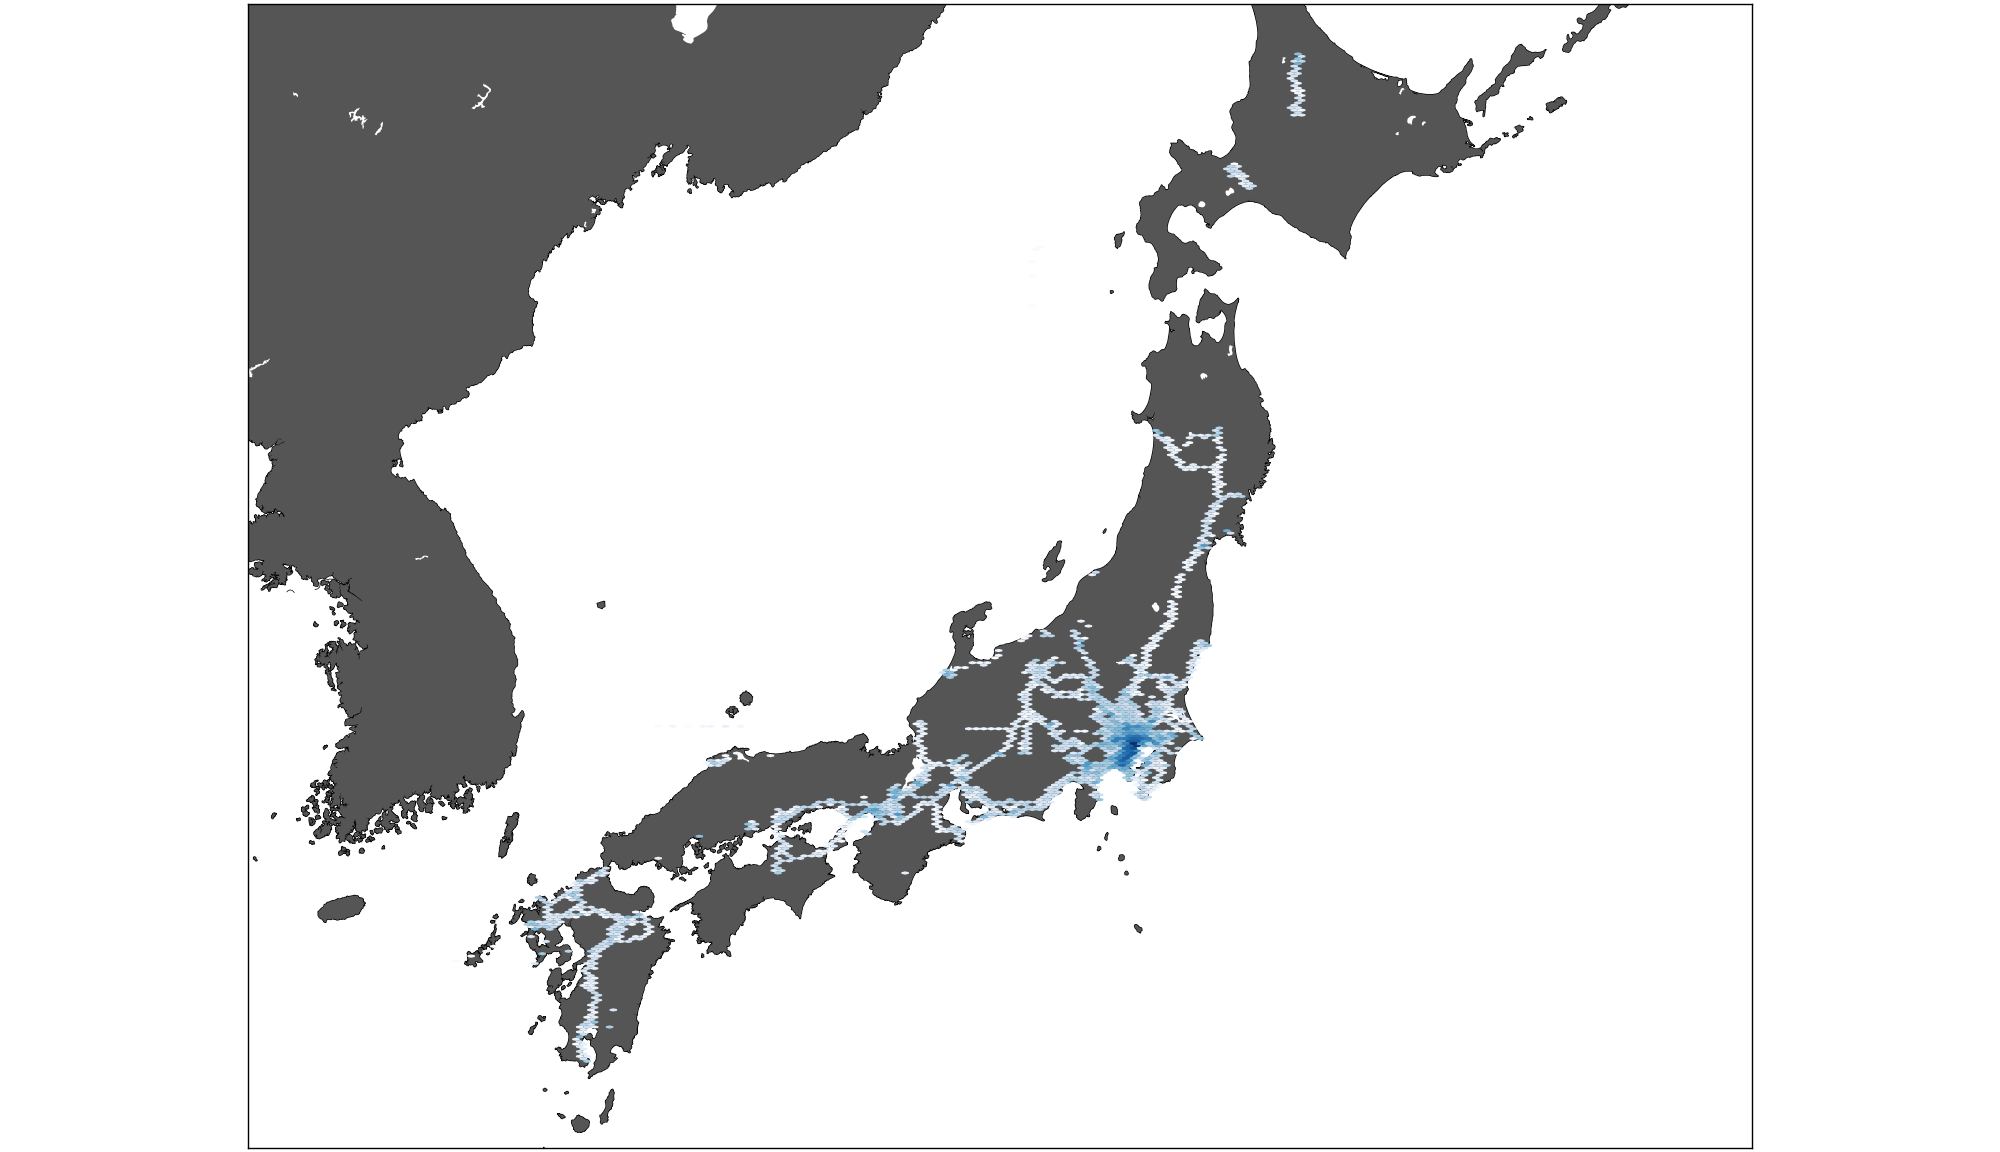
\includegraphics[scale=0.30]{all_locations_japan}
    \caption{Location updates in Japan, hexbinned}
    \label{fig:japan_locations_hexbin}
\end{figure}

\section{Modeling}
In this subsection we will describe the model and features used for prediction.

We will try to answer the following question: Can we predict if people meet in a period based on their spatiotemporal patterns in a previous period.
The models and algorithms we use are implemented in \textit{scikit-learn}\cite{scikit-learn} a Python module for machine learning. 

First we will describe the different features of which our dataset is composed.
\subsection{Features}
\subsubsection{Number of co-occurrences (num\_coocs)}
The total number of co-occurrences between users.
\subsubsection{Diversity of a co-occurrence}
We use the diversity measure taken from the papers of Shahabi and Pham\cite{iRWRfSD}\cite{AEBMtISSfSD}.
Diversity is a measure of how important the spatial locations of the co-occurrences between a pair of persons are, given how many times they appear.
It exists in two forms, one using Shannon entropy another using Rényi entropy, we will use Shannon.
The Shannon entropy is defined by Equation \ref{eq:shannon_entropy}
\begin{equation}
\label{eq:shannon_entropy}
H^S_{ij}=-\sum\limits_{l}P^l_{ij} \log P^l_{ij}= -\sum\limits_{l,c_ij,l\neq 0}\frac{c_{ij,l}}{f_{ij}}\log \frac{c_{ij,l}}{f_{ij}}
\end{equation}
where $f_{ij}$, the \textit{frequency}, is the total number of co-occurrences between user $i$ and user $j$, and $c_{ij,l}$, the \textit{local frequency}, is the total number of co-occurrences between user $i$ and $j$ at location $l$.
From this the diversity is defined by taking the exponential function of the entropy defined in Equation \ref{eq:diversity}:
\begin{equation}
\label{eq:diversity}
D^s_{ij} = exp(H^S_{ij})
\end{equation}

\subsubsection{Weighted frequency}
We use the weighted frequency measure taken from the papers of Shababi and Pham\cite{iRWRfSD}\cite{AEBMtISSfSD}.
Weighted frequency is a measure of how important the co-occurrences at non-popular places are.
The weighed frequency is defined by Equation \ref{eq:weighted_frequency}
\begin{equation}
\label{eq:weighted_frequency}
F_{ij}=\sum\limits_{l}c_{ij,l} \times \exp(-H_l)
\end{equation}
where $H_l$ is the Location Entropy for location \textit{l} defined in Equation \ref{eq:location_entropy}
\begin{equation}
\label{eq:location_entropy}
H_l = \sum\limits_{u, P_{u,l}\neq0} P_{u,l}\log P_{u,l}
\end{equation}
where $P_{u,l}$ is the probability that a location update from location \textit{l} belongs to user \textit{u}.
\subsubsection{Co-occurrences weighted with respect to each location}
We use the weighted co-occurrences measure taken from the master's thesis of P. Sapieżyński\cite{IMM2013-06556}.

\subsubsection{Timely arrival and leaving}
We use the timely arrival and leaving measure taken from the master's thesis of P. Sapieżyński\cite{IMM2013-06556}.

\subsubsection{Unique spatial bins}
The number of unique spatial bins between two users.

\subsubsection{Jaccard index similarity of used apps}
The Jaccard index is a measure used in comparing the similarity of sample sets. We extract what apps two users have used in the period and compute the similarity between them using the Jaccard index.
The Jaccard index is defined in Equation \ref{eq:jaccard_index}
\begin{equation}
\label{eq:jaccard_index}
J(A_i,A_j) = \frac{ |A_i \cap A_j| }{ |A_i \cup A_j | }
\end{equation}
where $A_i$ is the set of apps used by user $i$ and $A_j$ is the set of apps used by user $j$. If $A_i$ and $A_j$ are empty sets we define $J(A_i, A_j) = 1$

\subsection{Results}
For our training set we found 124 negative samples (did not meet) and 2331 positive samples (did meet), the high number of positive samples is due to the inclusion of Sony HQ location updates in our training set. In our test set we found a more moderate 289 negative samples (did not meet) and 191 positive samples (did meet).
First we trained a Logistic Regression classifier which serves as our baseline classifier to compare our other model with. We trained it only with the feature num\_coocs. Next we trained a Random Forest classifier with all of our features.

\subsection{Performance metrics}
We utilized the precision and recall metrics for evaluating the performance of our models as well as AUC of the ROC Curve.
\subsubsection{Precision}

\subsubsection{Recall}

\subsubsection{ROC AUC}

In Table \ref{table:models_performance_report} we can see the performance metrics for the positive class (did meet).

\begin{table}[htbp]
\centering
\begin{tabular}{|c|c|c|c|c|c|c|c|c|c|c|}
\hline
\textbf{Model} & \textbf{Precision - positive} & \textbf{Recall - positive} & \textbf{Precision - negative} & \textbf{Recall - negative}   \\
\hline
Logistic Regression (num\_coccs)          & 0.86 & 0.03 & 0.00 & 0.00       \\
\hline
Random Forest (T = 10)    & 0.49 & 0.57 & 0.68 & 0.62\\
\hline
Logistic Regression (num\_coocs, balanced class weight)          & 0.86 & 0.03 & 0.61 & 1.00      \\
\hline
Random Forest (balanced class weight, T = 200)    & 0.44 & 0.79 & 0.71 & 0.34\\
\hline
\end{tabular}
\caption{Models performance metrics for the positive class (did meet)}
\label{table:models_performance_report}
\end{table}



\subsection{Class Imbalance Problem}
The Class Imbalance Problem is when the total number of data for one class greatly exceeds the number of data for a different class.


